\chapter[Casos de Uso]{Casos de Uso}

\section{Diagrama de Casos de Uso}

\begin{figure}[h!]
	\begin{center}
		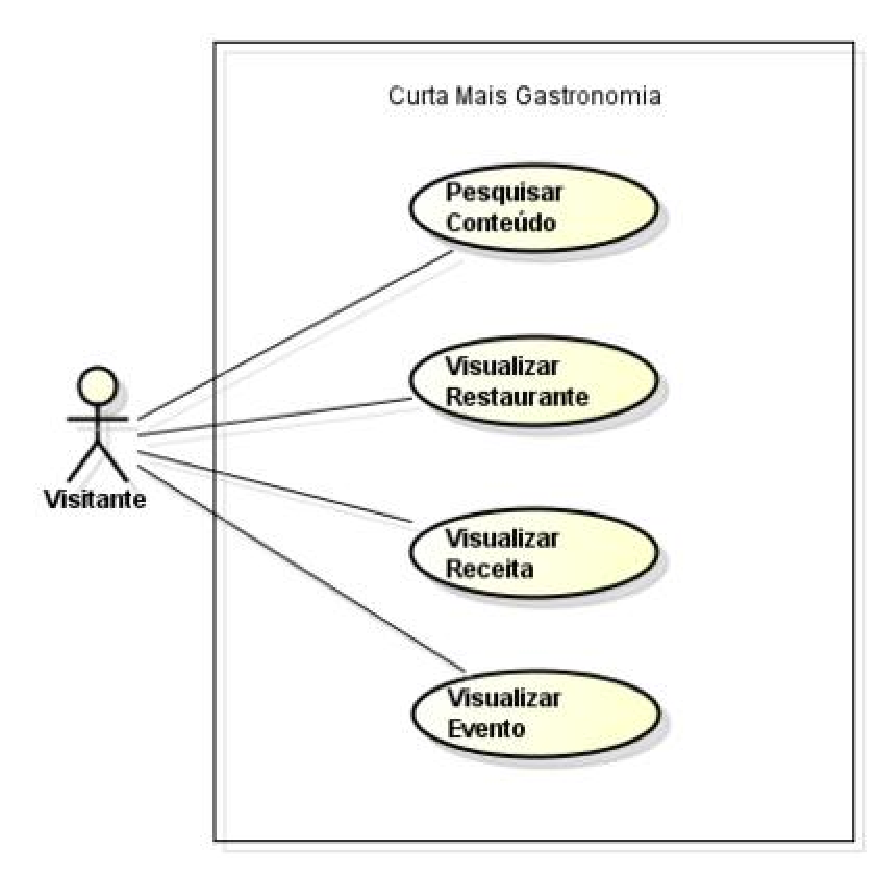
\includegraphics[keepaspectratio,scale=0.6]{figuras/diagrama.eps}
		\caption{Diagrama de Caso de Uso - Gastronomia}
	\end{center}
\end{figure}

\section{Descrição dos Casos de Uso}

\begin{table}[t]
\begin{tabular}{| p{6cm} | p{10cm} |}
	\hline
	\textbf{ID} & UC02\tabularnewline
	\hline
	\hline
	\textbf{Nome do Caso de Uso} & Visualizar Restaurante\tabularnewline
	\hline
	\textbf{Objetivo} & Apresentar detalhes de um restaurante para o visitante\tabularnewline
	\hline
	\textbf{Ator(es)} & Visitante\tabularnewline
	\hline
	\textbf{Pré-condição} & Acessar a aplicação\tabularnewline
	\hline
	\textbf{Pós-condição} & \tabularnewline
	\hline
	\textbf{Fluxo Principal /Básico /Normal} & \textbf{Este caso de uso se inicia quando o visitante seleciona a opção de restaurantes:}
	\vspace{0.2cm}
	\begin{enumerate}
		\item O visitante clica em uma categoria de restaurante.
		\item O sistema encaminha o visitante para uma lista de restaurantes sob aquela categoria.
		\item O visitante clica no nome de um dos restaurantes listados.
		\item O sistema encaminha o visitante para a página do restaurante selecionado.
		\item Este caso de uso é encerrado.
	\end{enumerate} \tabularnewline
	\hline
	\textbf{Fluxo Alternativo} & \textbf{Fluxo alternativo de voltar para tela anterior:}
	\vspace{0.2cm}
	Este fluxo se inicia quando o visitante decide voltar para a tela anterior do sistema.
	\begin{enumerate}
		\item O visitante seleciona o botão “VOLTAR”.
		\item O sistema encaminha o visitante para a página anterior do sistema.
		\item Este caso de uso é encerrado.
	\end{enumerate} \tabularnewline
	\hline
\end{tabular}
\caption{Descricao dos Casos de Uso - Visualizar Restaurante}
\label{DCU_Vizualizar_Restaurante}
\end{table}


\begin{table}[t]
\begin{tabular}{| p{6cm} | p{10cm} |}
	\hline
	\textbf{ID} & UC02\tabularnewline
	\hline
	\hline
	\textbf{Nome do Caso de Uso} & Visualizar Receita\tabularnewline
	\hline
	\textbf{Objetivo} & Apresentar detalhes de uma receita para o visitante\tabularnewline
	\hline
	\textbf{Ator(es)} & Visitante\tabularnewline
	\hline
	\textbf{Pré-condição} & Acessar a aplicação\tabularnewline
	\hline
	\textbf{Pós-condição} & \tabularnewline
	\hline
	\textbf{Fluxo Principal /Básico /Normal} & \textbf{Este caso de uso se inicia quando o visitante seleciona a opção de restaurantes:}
	\vspace{0.2cm}
	\begin{enumerate}
		\item O visitante clica em uma categoria de receita.
		\item O sistema encaminha o visitante para uma lista de receitas sob aquela categoria.
		\item O visitante clica no nome de uma das receitas listadas.
		\item O sistema encaminha o visitante para a página da receita selecionada.
		\item Este caso de uso é encerrado.
	\end{enumerate} \tabularnewline
	\hline
	\textbf{Fluxo Alternativo} & \tabularnewline
	\hline
	\textbf{Fluxo Alternativo} & \textbf{Fluxo alternativo de voltar para tela anterior:}
	\vspace{0.2cm}
	Este fluxo se inicia quando o visitante decide voltar para a tela anterior do sistema.
	\begin{enumerate}
		\item O visitante seleciona o botão “VOLTAR”.
		\item O sistema encaminha o visitante para a página anterior do sistema.
		\item Este caso de uso é encerrado.
	\end{enumerate} \tabularnewline
	\hline
\end{tabular}
\caption{Descricao dos Casos de Uso - Visualizar Receita}
\label{DCU_Visualizar_Receita}
\end{table}

\begin{table}[t]
\begin{tabular}{| p{6cm} | p{10cm} |}
	\hline
	\textbf{ID} & UC03\tabularnewline
	\hline
	\hline
	\textbf{Nome do Caso de Uso} & Visualizar Evento\tabularnewline
	\hline
	\textbf{Objetivo} & Apresentar detalhes de uma evento para o visitante\tabularnewline
	\hline
	\textbf{Ator(es)} & Visitante\tabularnewline
	\hline
	\textbf{Pré-condição} & Acessar a aplicação\tabularnewline
	\hline
	\textbf{Pós-condição} & \tabularnewline
	\hline
	\textbf{Fluxo Principal /Básico /Normal} & \textbf{Este caso de uso se inicia quando o visitante seleciona a opção de eventos:}
	\vspace{0.2cm}
	\begin{enumerate}
		\item O visitante clica em um dos eventos listados.
		\item O sistema encaminha o visitante para a página do evento selecionado.
		\item Este caso de uso é encerrado.
	\end{enumerate} \tabularnewline
	\hline
	\textbf{Fluxo Alternativo} & \tabularnewline
	\hline
	\textbf{Fluxo Alternativo} & \textbf{Fluxo alternativo de voltar para tela anterior:}
	\vspace{0.2cm}
	Este fluxo se inicia quando o visitante decide voltar para a tela anterior do sistema.
	\begin{enumerate}
		\item O visitante seleciona o botão “VOLTAR”.
		\item O sistema encaminha o visitante para a página anterior do sistema.
		\item Este caso de uso é encerrado.
	\end{enumerate} \tabularnewline
	\hline
\end{tabular}
\caption{Descricao dos Casos de Uso - Visualizar Evento}
\label{DCU_Visualizar_Evento}
\end{table}

\begin{table}[t]
\begin{tabular}{| p{6cm} | p{10cm} |}
	\hline
	\textbf{ID} & UC04\tabularnewline
	\hline
	\hline
	\textbf{Nome do Caso de Uso} & Buscar Conteúdo\tabularnewline
	\hline
	\textbf{Objetivo} & Retornar conteúdo específico solicitado pelo visitante\tabularnewline
	\hline
	\textbf{Ator(es)} & Visitante\tabularnewline
	\hline
	\textbf{Pré-condição} & Acessar a aplicação\tabularnewline
	\hline
	\textbf{Pós-condição} & \tabularnewline
	\hline
	\textbf{Fluxo Principal /Básico /Normal} & \textbf{Este caso de uso se inicia quando o visitante realiza uma busca na aplicação:}
	\vspace{0.2cm}
	\begin{enumerate}
		\item O sistema retorna uma lista com conteúdos que contenham o termo pesquisado.
		\item O visitante clica em um dos conteúdos retornados.
		\item O sistema encaminha o visitante para a página daquele conteúdo.
		\item Este caso de uso é encerrado.
	\end{enumerate} \tabularnewline
	\hline
	\textbf{Fluxo Alternativo} & \tabularnewline
	\hline
	\textbf{Fluxo Alternativo} & \textbf{Fluxo alternativo de filtragem de resultados:}
	\vspace{0.2cm}
	Este fluxo começa quando o visitante seleciona algum filtro para refinar a pesquisa no site.
	\begin{enumerate}
		\item O visitante clica em um dos filtros da busca.
		\item O sistema retorna resultados que pertençam apenas à(s) categoria(s) filtrada(s).
		\item O visitante clica em um dos conteúdos retornados.
		\item Este caso de uso é encerrado.
	\end{enumerate}

	\textbf{Fluxo alternativo de voltar para tela anterior:}
	\vspace{0.2cm}
	Este fluxo se inicia quando o visitante decide voltar para a tela anterior do sistema.
	\begin{enumerate}
		\item O visitante seleciona o botão “VOLTAR”.
		\item O sistema encaminha o visitante para a página anterior do sistema.
		\item Este caso de uso é encerrado.
	\end{enumerate} \tabularnewline
	\hline
\end{tabular}
\caption{Descricao dos Casos de Uso - Visualizar Evento}
\label{DCU_Visualizar_Evento}
\end{table}